\documentclass[document.tex]{subfiles}
\begin{document}

\chapter{Introduction}
\section{Introduction}
Newspaper articles on stock prices, business news, several advertising on product’s current rate, and offers on products of
super shops are described in Natural Language. Even Sports
commentaries, election results, modern Chat bots for Questions
and Answers are also in Natural Language.Computers, since their creation, have exceeded human beings in (speed and accuracy of) mathematical calculation. However, it is still a big challenge nowadays to design algorithms to automatically solve several percentage related problems or context. We need an algorithm to solve those percentage word problems.

\section{Math Word Problem}
\noindent Mathematical Problems that are described in human language called Math Word Problems. There are many types of math word problems. Such as- Addition Word Problems, Subtraction Word Problems, Multiplication Word Problems, Division Word Problems, Percentage Word Problem etc.

In the following subsection, we have discussed about the Percentage word Problem with an example:
\subsection{Percentage Word Problem}
\noindent Percentage Word Problems are the mathematical problems that are also described in natural language or human like language and it contains the word or mathematics related to ``Percentage Problems". Sometimes it contains the system of percentage(\%). Figure \ref{fig:a} shows an example of Percentage Word Problem.
\begin{figure}[H] 
	\fbox{
		\begin{minipage}{0.97\textwidth}
			
			The height of a mountain on a tropical island changes due to volcanic activity. When the mountain was last measured, its height was 3,750 meters. Now it is \textbf{10\% taller}. How tall is the mountain currently?
			
		\end{minipage}
	}
	\caption{Example of a Percentage Word Problem}
	\label{fig:a}
\end{figure}

In Figure \ref{fig:a}, \textbf{10\%} is the phrase by which we can recognize the percentage word problems. In all the percentage problem, the word ``\textbf{Percentage}'' or symbol ``\textbf{\%}'' is always present.

\section{Parsing}
Understanding natural language text, it always need parsing. Parsing is the process of analyzing a string of symbols, either in natural language or in computer languages, conforming to the rules of a formal grammar. The term parsing comes from Latin pars (orationis), meaning part (of speech).

The term has slightly different meanings in different branches of linguistics and computer science. Traditional sentence parsing is often performed as a method of understanding the exact meaning of a sentence or word, sometimes with the aid of devices such as sentence diagrams. It usually emphasizes the importance of grammatical divisions such as subject and predicate.
Parsing are basically two types. One is \textbf{syntax analysis} and other is \textbf{semantic analysis}. Syntax Analysis is based on verb count and semantic analysis based on the meaning of the sentence.

A \textbf{parser} is a software component that takes input data (frequently text) and builds a data structure – often some kind of parse tree, abstract syntax tree or other hierarchical structure – giving a structural representation of the input, checking for correct syntax in the process. The parsing may be preceded or followed by other steps, or these may be combined into a single step. The parser is often preceded by a separate lexical analyser, which creates tokens from the sequence of input characters; alternatively, these can be combined in scannerless parsing. Parsers may be programmed by hand or may be automatically or semi-automatically generated by a parser generator. Parsing is complementary to templating, which produces formatted output. These may be applied to different domains, but often appear together, such as the scanf/printf pair, or the input (front end parsing) and output (back end code generation) stages of a compiler. The overview of the parsing is shown in the figure below:
\begin{figure}[H]
	\begin{center}
		\begin{tikzpicture}[node distance=1.5cm]
		% Place nodes
		\node [startstop] (SS) {Source String};
		\node [process,  below of= SS] (LA) {Lexical Analysis (Create Tokens)};
		\node [startstop, below of =  LA] (TK) {Tokens};
		\node [process, below of=  TK] (SA) {Syntactic Analysis};
		\node [startstop, below of=SA] (PT) {Parse Tree};
		\node [process, below of=  PT] (CIT){Compiler, Interpreter or Translator};
		\node [startstop, below of = CIT] (OP){Output};
		
		% Draw edges
		\draw [arrow] (SS) -- (LA);
		\draw [arrow] (LA) -- (TK);
		\draw [arrow] (TK) -- (SA);
		\draw [arrow] (SA) -- (PT);
		\draw [arrow] (PT) -- (CIT);
		\draw [arrow] (CIT) -- (OP);
		
		\end{tikzpicture}
	\end{center}
	\caption{Flowchart of Parser\cite{wikiparsing}}
	\label{fig:flowchart}
\end{figure}
%	\begin{center}
%		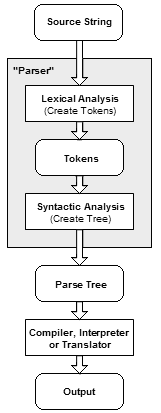
\includegraphics[height=13.0cm]{imgs/Parser.png}
%	\end{center}
%\end{figure}
\section{Background}
\noindent Automatically solving Math Word Problem is a recently hot topic on understanding Natural Language. However, actual journey of solving was started from the 1960s. Algebraic problems of Natural Language was transformed into kernel sentences and handles to solve the problems in STUDENT\cite{4}. In CARPS\cite{5}, they use pattern matching based on expressions by the transformed kernel sentences. However, they were limited to rate based problems. In \cite{6}, they first introduced tree-based structure to represent the information in the problem. Recent automatically solving math word problems include number word problems\cite{7}, logic puzzle problems\cite{8}, geometry word problems\cite{9,10}, arithmetic word problems\cite{1}, \cite{11} and algebra word problems\cite{2,3}, \cite{12}.

In the following subsections, we have discussed the related works in details:
\subsection{Semantic Parsing}
\noindent Semantic parsing is the process of mapping a natural-language sentence into a formal representation of its meaning. Semantics concerns its meaning: rules that go beyond mere
form (e.g., the number of arguments contained in a call to a
subroutine matches the number of formal parameters in the
subroutine definition – cannot be counted using Context Free Grammar, type
consistency):
\begin{itemize}
	\item Defines what the program means
	\item Detects if the program is correct
	\item Helps to translate it into another representation
\end{itemize}
In semantic parsing, there have been many works. Language grounding for interpretation of a sentence in world representation has related to many works \cite{13, 14, 15, 16, 17, 18, 19, 20, 21, 22, 23}. We discuss three pioneering work closely related to our work.
\subsection{Verb Categorization Technique}
\noindent In \cite{1}, they tried to solve addition and subtraction problems by verb categories to update a world representation derived from problem text. They ground the problem text to semantic entities and containers. Based on learned verb categories, their system works well for addition and subtraction.
They investigates the task of learning to
solve such problems by mapping the verbs in the
problem text into categories that describe their im-
pact on the world state. While the verbs category
is crucial, some elements of the
problem are irrelevant. For instance, the fact that
three kittens have spots is immaterial to the solution. 
%Overview of the process of verb categorization is shown below:
%\begin{figure}[H]
%	\begin{center}
%		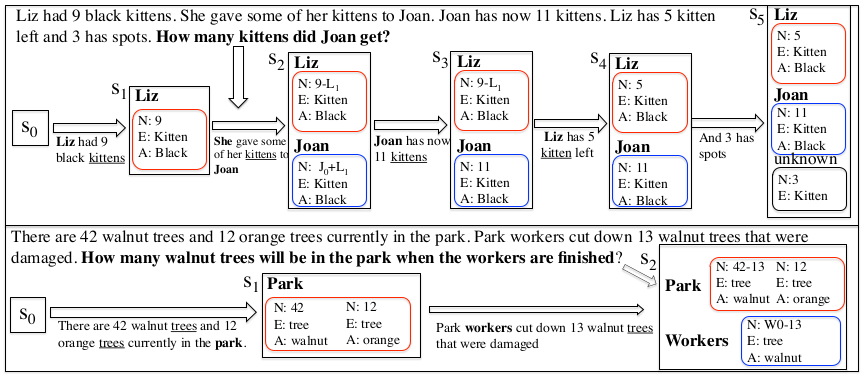
\includegraphics[height=10cm, width=16cm]{imgs/Verb.jpg}
%	\end{center}
%\end{figure}
\subsection{Template Matching Technique}
\noindent In \cite{2}, they introduce a general method for solving algebra problems. This work can align a word problem to a system of equations with one or two unknowns. They learn a mapping from word problems to equation templates using global and local features from the problem text. However, the
large space of equation templates makes it challenging for this model to learn to find the best equation
directly, as a sufficiently similar template may not
have been observed during training.
\subsection{Hybrid of Verb Categorization and Template Matching Technique}
\noindent In ALGES\cite{3}, they tried to solve the problem of solving multiple sentenced algebraic word problems by generating and ranking the equation trees. They use a richer semantic representation of the problem text and a bottom-up approach to learning the relations between spans of texts and arithmetic operators. Then score the equations using a global form of the problem to produce the final result. ALGES combined the previous methods to use in broader scope like, Addition, Subtraction, Multiplication and Division for solving single variable problems.

ALGES learns to map spans of text to arithmetic operators, to combine them given the global context of the problem, and to
choose the “best” tree corresponding to the problem.
The training set for ALGES consists of unannotated
algebraic word problems and their solution. Solving the equation represented by such a tree is trivial.
ALGES is able to solve word problems with single-variable equations.
In contrast to \cite{1} ALGES covers $ +, -, *, $ and $/$. The work of \cite{2} has broader scope but we show that it relies heavily on overlap between training and test data.

\section{Motivation}
Everyday life as a human being is very much related to percentage word problems. It starts from business to income of a person. 
\begin{figure}[H]
	\begin{multicols}{4}[\columnsep=2.0cm]
		
\includegraphics[scale=0.55]{imgs/news.png}
		\columnbreak
		
		
\includegraphics[scale=0.15]{imgs/stock.png}
		\columnbreak
		
		
\includegraphics[scale=0.092]{imgs/product_prices.png}
		\columnbreak
		
		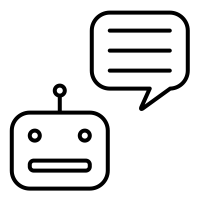
\includegraphics[scale=0.35]{imgs/chatbot.png}
		
	\end{multicols}
	\caption {Related to Percent Word Problems\cite{googleimage}}
	\label{fig:relatedFig}
\end{figure}
In Figure \ref{fig:relatedFig}, some related problems related to daily life of human is shown. Here is some dots of percentage word problems-
\begin{itemize}
	\item  Newspaper Articles report statistics to present stock prices analysis,
	\item  Market Analysis for products current rate,
	\item  Sport Commentaries, Financial News,
	\item  Chatbots for Question and Answering System,
	\item Income tax calculation,
	\item Increment on Salary,
	\item Utility Bills etc.
\end{itemize}
So, its badly needed a system that could solve those problems of daily life efficiently.

\section{Objectives}

Solving Word Problems requires semantic parsing and reasoning across sentence to find equations. In our system, we have used verb categorization to ground the problem text and divide them entities, containers, and quantities by semantic parsing. After that we have mapped possible equation trees based on those.

In previous, math word problems are tried to solve with verb categorization \cite{1} and template based method \cite{2}. ALGES \cite{3} is a hybrid method which combines both verb categorization and template-based method for solving single variable addition, subtraction, multiplication and division problems.

Our work is related to ALGES, where we converted the percent related number to a fraction and force the problem text to covert it like the problem for ALGES. That is related to using ILP to enforce global constraints in NLP applications\cite{24}. Like previous\cite{25, 26, 27, 28}, ALGES used ILP to form candidate equations which are then used to generate training data for classification. ALGES attempts to parser re-rank the equations\cite{29, 30}.

\noindent In this system, we have the following objectives:
\begin{itemize}
	\item Build a new dataset for Percentage Word Problems,
	\item Introduce a new scoring equation, and
	\item Solving Percentage Word Problems.
\end{itemize}

%\section{What's in our system?}
%In our system, we have used ALGES to a broader scope to solve percentage word problems. We have converted the problem text first. Then generate equation trees by semantic parsing and \textbf{Integer Linear Programming (ILP)} to solve the problem. 
%
%In training, we train local relationship model from the generated equations and their results to set an operator between two operands and a global model based on the equations solution label by correct or incorrect. 
%
%In testing, set a score for the generated equations from the local and global model and choose the equation with the highest score as the final equation for a problem text.

\section{Contributions}
\noindent Our contributions for solving percentage word problems are as follows: 
\begin{enumerate}
	\item We have converted and preprocessed the problem text like, addition, subtraction, multiplication and division problems from the percentage problems; 
	\item A new scoring equation for generating solutions;
	\item A newly build efficient dataset on Percentage Word Problems; 
	\item Finally, a system \textbf{Percentage Word Problem Solver} named as \textbf{PWPS} that can solve 69.19\% Percentage Word Problems.
\end{enumerate}

\section{Organization of Thesis}
\noindent \textbf{Chapter 2} is dedicated for the methodology of the system in details. Flowchart, Algorithm are described section by section. In the subsection, Constructing Tree, Generating Equation and Testing and Training methods are described. Sample description about Random Forests classifier is given.

\noindent \textbf{Chapter 3} depicts the experimental evaluation of the system. Dataset, experimental setup are described in details in this chapter. Implementation procedure and cross-validation are also discussed in this chapter.


\noindent \textbf{Chapter 4} is dedicated for the evaluation matrix, result and the performance analysis. It contains Comparison, Ablation Study and Error Analysis.


\noindent \textbf{Chapter 5} represents the summary of this research work and highlights the overall contribution. A direction also given on the future scope of math word problem solving.


\noindent \textbf{Appendix A} presents the system installation details.

\end{document}
